% ------------------------------------------------------------------------------
% TYPO3 CMS 6.2 LTS - What's New - Chapter "In-Depth Changes" (Russian Version)
%
% @author	Andrey Aksenov <aksenovaa@bk.ru>
% @license	Creative Commons BY-NC-SA 3.0
% @link		http://typo3.org/download/release-notes/whats-new/
% @language	Russian
% ------------------------------------------------------------------------------
% Chapter: In-Depth Changes
% ------------------------------------------------------------------------------

\section{Внутренние изменения}
\begin{frame}[fragile]
	\frametitle{Внутренние изменения}

	\begin{center}\huge{Глава 6:}\end{center}
	\begin{center}\huge{\color{typo3darkgrey}\textbf{Внутренние изменения}}\end{center}

\end{frame}

% ------------------------------------------------------------------------------
% normalize.css
% ------------------------------------------------------------------------------
% http://forge.typo3.org/issues/47920

\begin{frame}[fragile]
	\frametitle{Внутренние изменения}
	\framesubtitle{Normalize.css}

	\begin{itemize}
		\item Внутренний интерфейс использует \texttt{normalize.css},\newline
			что делает его единообразным во всех браузерах и приводит в соответствие к современными стандартами
		\item Современная, в стиле HTML5, альтернатива традиционным CSS reset
		\item Назначение \texttt{normalize.css}:

			\begin{itemize}
				\item Сохранение полезных начальных установок браузеров, вместо их переназначения
				\item Единообразие стилей для широкого диапазона элементов HTML
				\item Исправление ошибок и несоответствий в браузерах
				\item Улучшение удобства пользования
				\item Разъяснение кода при помощи комментариев и детальной документации
			\end{itemize}

	\end{itemize}

\end{frame}

% ------------------------------------------------------------------------------
% displayCond options BIT and !BIT
% ------------------------------------------------------------------------------
% http://forge.typo3.org/issues/45514

\begin{frame}[fragile]
	\frametitle{Внутренние изменения}
	\framesubtitle{TCA: displayCond параметры BIT и !BIT}

	\lstset{
		basicstyle=\tiny\ttfamily
	}

	\begin{itemize}
		\item Проверка при помощи многозначного поля в \texttt{displayCond} (bitwise)\newline
			\texttt{BIT}: бит установлен, \texttt{!BIT}: бит \underline{не} установлен
	\end{itemize}

	\begin{columns}[T]

		\begin{column}{.5\textwidth}

			\advance\leftskip+1cm
			Пример TCA:

			\lstset{xleftmargin=1cm}

			\begin{lstlisting}
				'content' => array(
				  'label' => '...',
				  'config' => array(
				    'type' => 'check',
				    'items' => array(
				      array('Content A', ''),
				      array('Content B', ''),
				      array('Content C', ''),
				    ),
				  )
				),
			\end{lstlisting}

		\end{column}
		\begin{column}{.5\textwidth}

			Примеры:

			\begin{lstlisting}
				'content_a' => array(
				  'label' => '...',
				  'displayCond' => 'FIELD:content:BIT:1',
				  'config' => array(
				    'type' => 'text',
				  )
				),

				'content_b' => array(
				  'label' => '...',
				  'displayCond' => 'FIELD:content:!BIT:2',
				  'config' => array(
				    'type' => 'text',
				  )
				),
			\end{lstlisting}
		\end{column}

	\end{columns}

\end{frame}

% ------------------------------------------------------------------------------
% Automatic language updates for extensions
% ------------------------------------------------------------------------------
% http://forge.typo3.org/issues/43703

\begin{frame}[fragile]
	\frametitle{Внутренние изменения}
	\framesubtitle{Обновления языков}

	\begin{itemize}
		% \item Extbase Command Controller allows to update translations of extensions for selected languages
		\item Extbase Command Controller позволяет обновлять переводы расширений:

			\begin{lstlisting}
				$GLOBALS['TYPO3_CONF_VARS']['SC_OPTIONS']['extbase']
				  ['commandControllers'][] =
				  'TYPO3\\CMS\\Lang\\Command\\LanguageCommandController';
			\end{lstlisting}

		\item Пример вызова:

			\lstinline!typo3/cli_dispatch.phpsh extbase language:update de,en,fr!

		\item Список локалей через запятую (например, \texttt{de,en,fr}) обновляет лишь указанные языки
		\item Без этого аргумента обновятся все языки, указанные в модуле "Языки"/"Languages"

	\end{itemize}

\end{frame}

% ------------------------------------------------------------------------------
% Migrate system extension manuals to reStructuredText
% ------------------------------------------------------------------------------
% http://forge.typo3.org/issues/50052

\begin{frame}[fragile]
	\frametitle{Внутренние изменения}
	\framesubtitle{Системные расширения: Руководства ReST}

	\begin{itemize}
		\item Все руководства для системных расширений используют reStructured Text
		\item Руководства в формате OpenOffice более не используются и удалены
		\item ReST – легкочитаемая и понятная система разметки с простым синтаксисом и анализатором
		\item Файлы ReST для системных расширений хранятся в:\newline
			\texttt{typo3/sysext/<extensionkey>/Documentation/*}

		\item Дополнительная информация:

			\begin{itemize}
				\item \url{http://de.wikipedia.org/wiki/ReStructuredText}
				\item \url{http://wiki.typo3.org/ReST}
			\end{itemize}

	\end{itemize}

\end{frame}

% ------------------------------------------------------------------------------
% Support custom translation servers for extensions
% ------------------------------------------------------------------------------
% http://forge.typo3.org/issues/50052

\begin{frame}[fragile]
	\frametitle{Внутренние изменения}
	\framesubtitle{Перевод на сторонних серверах}

	\begin{itemize}
		\item Реализована поддержка сторонних серверов переводов для расширений
		\item При помощи XLIFF и новых Сигнал/Слот (Signal/Slot),\newline
			это стало простой задачей (см. пример на следующем слайде)
		\item Возможное решение для сервера переводов: \textbf{Pootle}

			\begin{itemize}
				\item сетевой инструмент управления переводами с соответствующим интерфейсом
				\item написан на Python/Django
				\item оригинальная разработка и создание: \url{translate.org.za}
				\item лицензия GNU GPL
			\end{itemize}

	\end{itemize}

\end{frame}

% ------------------------------------------------------------------------------
% Support custom translation servers for extensions
% ------------------------------------------------------------------------------
% http://forge.typo3.org/issues/50052

\begin{frame}[fragile]
	\frametitle{Внутренние изменения}
	\framesubtitle{Перевод на сторонних серверах}

	Пример: \texttt{EXT:myextension/localconf.php}

	\lstset{
		basicstyle=\tiny\ttfamily
	}

	\begin{lstlisting}
		/**
		 * @var \TYPO3\CMS\Extbase\SignalSlot\Dispatcher $signalSlotDispatcher
		 */
		$signalSlotDispatcher =
		  \TYPO3\CMS\Core\Utility\GeneralUtility::makeInstance(
		    'TYPO3\\CMS\\Extbase\\SignalSlot\\Dispatcher');

		$signalSlotDispatcher->connect(
		  'TYPO3\\CMS\\Lang\\Service\\UpdateTranslationService',
		  'postProcessMirrorUrl',
		  'Company\\Extension\Slots\\CustomMirror',
		  'postProcessMirrorUrl'
		);
	\end{lstlisting}

\end{frame}

% ------------------------------------------------------------------------------
% Support custom translation servers for extensions
% ------------------------------------------------------------------------------
% http://forge.typo3.org/issues/50052

\begin{frame}[fragile]
	\frametitle{Внутренние изменения}
	\framesubtitle{Перевод на сторонних серверах}

	Пример: \texttt{EXT:myextension/Classes/Slots/CustomMirror.php}

	\lstset{
		basicstyle=\tiny\ttfamily
	}

	\begin{lstlisting}
		<?php
		namespace Company\Extensions\Slots;
		class CustomMirror {

		  /**
		   * @var string
		   */
		  protected static $extKey = 'myextension';

		  public function postProcessMirrorUrl($extensionKey, &$mirrorUrl) {
		    if ($extensionKey === self::$extKey) {
		      $mirrorUrl = 'http://example.com/typo3-packages/';
		    }
		  }

		}
	\end{lstlisting}

\end{frame}

% ------------------------------------------------------------------------------
% Support custom translation servers for extensions
% ------------------------------------------------------------------------------
% http://forge.typo3.org/issues/50052

\begin{frame}[fragile]
	\frametitle{Внутренние изменения}
	\framesubtitle{Перевод на сторонних серверах}

	Ожидаемая структура файлов/директорий на сервере:

	\begin{lstlisting}
		http://example.com/typo3-packages/
		 `-- <first-letter-of-extension-key>
		     `-- <second-letter-of-extension-key>
		         `-- <extension-key>-l10n
		             |-- <extension-key>-l10n-de.zip
		             |-- <extension-key>-l10n-fr.zip
		             |-- <extension-key>-l10n-it.zip
		             `-- <extension-key>-l10n.xml
	\end{lstlisting}

	Для примера:

	\begin{lstlisting}
		http://example.com/typo3-packages/m/y/myextension-l10n/myextension-l10n.xml
	\end{lstlisting}

\end{frame}

% ------------------------------------------------------------------------------
% Support custom translation servers for extensions
% ------------------------------------------------------------------------------
% http://forge.typo3.org/issues/50052

\begin{frame}[fragile]
	\frametitle{Внутренние изменения}
	\framesubtitle{Перевод на сторонних серверах}

	Пример: \texttt{<extension-key>-l10n.xml}

	\lstset{
		basicstyle=\tiny\ttfamily
	}

	\begin{lstlisting}
		<?xml version="1.0" standalone="yes" ?>
		  <TERlanguagePackIndex>
		    <meta>
		      <timestamp>1374841386</timestamp>
		      <date>2013-07-26 14:23:06</date>
		    </meta>
		    <languagePackIndex>
		    <languagepack language="de">
		      <md5>1cc7046c3b624ba1fb1ef565343b84a1</md5>
		    </languagepack>
		    <languagepack language="fr">
		     <md5>f00f73ae5c43cb68392e6c508b65de7a</md5>
		    </languagepack>
		    <languagepack language="it">
		     <md5>cd59530ce1ee0a38e6309544be6bcb3d</md5>
		    </languagepack>
		  </languagePackIndex>
		</TERlanguagePackIndex>
	\end{lstlisting}

\end{frame}

% ------------------------------------------------------------------------------
% Automatic import of t3d files for extensions
% ------------------------------------------------------------------------------
% http://forge.typo3.org/issues/51437

\begin{frame}[fragile]
	\frametitle{Внутренние изменения}
	\framesubtitle{Автоматический импорт t3d}

	\begin{itemize}
		\item Теперь расширения могут автоматически импортировать исходные \textbf{t3d пакеты}\newline
			во время установки
		\item Файлы t3d содержат данные, связи, файлы и т. п.
		\item Файлы t3d должны иметь названия \texttt{data.t3d} и быть расположены в:\newline
			\texttt{EXT:myextension/Initialisation/}

		\item Импорт осуществляется лишь \underline{единожды}\newline
			(даже при последующей переустановке расширения)

	\end{itemize}

\end{frame}

% ------------------------------------------------------------------------------
% Automatic import of files for extensions
% ------------------------------------------------------------------------------
% http://forge.typo3.org/issues/51446

\begin{frame}[fragile]
	\frametitle{Внутренние изменения}
	\framesubtitle{Автоматический импорт файлов}

	\begin{itemize}
		\item Теперь расширения могут автоматически импортировать исходные \textbf{файлы}\newline
			во время установки
		\item Файлы должны быть расположены в:\newline
			\texttt{EXT:myextension/Initialisation/Files/...}
		\item Файлы копируются в:\newline
			\texttt{fileadmin/<extensionkey>/}
		\item Импорт осуществляется лишь \underline{единожды}\newline
			(даже при последующей переустановке расширения)

	\end{itemize}

\end{frame}

% ------------------------------------------------------------------------------
% Use an extension as repository
% ------------------------------------------------------------------------------
% http://forge.typo3.org/issues/51835

\begin{frame}[fragile]
	\frametitle{Внутренние изменения}
	\framesubtitle{Использование расширения в качестве репозитория}

	\begin{itemize}
		\item Иногда расширения зависят от определённой версии другого расширения, не имеющейся в официальном репозитории
		расширений TYPO3 (TYPO3 Extension Repository – TER)
		\item Для разрешения подобных проблем, теперь расширения могут поставляться с "другими" расширениями
		\item Они должны быть расположены в (распакованные):\newline
			\texttt{EXT:myextension/Initialisation/Extensions/...}

		\item В процессе установки они копируются в:\newline
			\texttt{typo3conf/ext/}

		\item Тем самым разрешается зависимость от сторонних расширений

	\end{itemize}

\end{frame}

% ------------------------------------------------------------------------------
% CLI command to install/uninstall extensions
% ------------------------------------------------------------------------------
% http://forge.typo3.org/issues/51629

\begin{frame}[fragile]
	\frametitle{Внутренние изменения}
	\framesubtitle{Установка/удаление расширений через CLI}

	\begin{itemize}
		\item Расширения можно установить или удалить через интерфейс командной строки (CLI)
		\item Примеры:
			\lstinline!typo3/cli_dispatch.phpsh extbase extension:install <extensionkey>!
			\lstinline!typo3/cli_dispatch.phpsh extbase extension:uninstall <extensionkey>!

		\item Замечание: для этого необходимо наличие внутреннего пользователя \textbf{\_cli\_lowlevel}
	\end{itemize}

\end{frame}

% ------------------------------------------------------------------------------
% Enable/disable cascading deletion of child elements
% ------------------------------------------------------------------------------
% http://forge.typo3.org/issues/50391

\begin{frame}[fragile]
	\frametitle{Внутренние изменения}
	\framesubtitle{Каскадное удаление дочерних элементов}

	\begin{itemize}
		\item В TCA добавлен параметр для включения/отключения каскадного удаления дочерних элементов
		\item Тип связи должен быть "inline"
		\item Значение по умолчанию \texttt{TRUE} (включено каскадное удаление дочерних элементов)
		\item Пример (отключение удаления дочерних записей):

			\begin{lstlisting}
				...
				'type' => 'inline',
				'foreign_table' => ...,
				  'behaviour' => array(
				    'enableCascadingDelete' => 0
				  )
				  ...
				)
				...
			\end{lstlisting}

	\end{itemize}

\end{frame}

% ------------------------------------------------------------------------------
% Multiple category fields per table
% ------------------------------------------------------------------------------
% http://forge.typo3.org/issues/51921

\begin{frame}[fragile]
	\frametitle{Внутренние изменения}
	\framesubtitle{Поля для нескольких категорий для таблицы}

	\begin{itemize}
		\item В TYPO3 < 6.2, был возможен лишь \underline{один} \texttt{makeCategorizable()} вызов для таблицы
			(несколько вызовов переназначают предыдущее назначение категории)
		\item Начиная с TYPO3 >= 6.2, для таблицы возможны несколько категорий
		\item Пример:

			\begin{lstlisting}
				\TYPO3\CMS\Core\Utility\ExtensionManagementUtility::makeCategorizable(
				  $extensionKey,
				  $tableName,
				  $fieldName = 'categories',
				  $options = array(
				  	'label' => 'my category'
				  )
				);
			\end{lstlisting}

		\item Свои мети для каждого из поле категорий возможно назначить в массиве 
		\texttt{\$options}

	\end{itemize}

\end{frame}

% ------------------------------------------------------------------------------
% Backend layout data providers
% ------------------------------------------------------------------------------
% http://forge.typo3.org/issues/37208

\begin{frame}[fragile]
	\frametitle{Внутренние изменения}
	\framesubtitle{Поставщики данных для шаблона внутреннего интерфейса}

	\begin{itemize}
		\item В TYPO3 < 6.2, шаблоны внутреннего интерфейса хранились в БД как обычные записи
		\item Начиная с TYPO3 >= 6.2, возможно определить так называемых \emph{поставщиков данных - data providers}.\newline
			\small(например, для возможности определения в расширении собственного внутреннего шаблона в расширении через 
			статические файлы)
			\normalsize

		\item Поставщики данных должны реализовывать интерфейс:\newline
			\smaller\texttt{
				TYPO3\textbackslash\textbackslash
				CMS\textbackslash\textbackslash
				Backend\textbackslash\textbackslash
				View\textbackslash\textbackslash
				BackendLayout\textbackslash\textbackslash
				DataProviderInterface}\normalsize

		\item и регистрироваться через:

			\begin{lstlisting}
				$GLOBALS['TYPO3_CONF_VARS']['SC_OPTIONS']
				  ['BackendLayoutDataProvider'][$_EXTKEY] = 'Classname';
			\end{lstlisting}


	\end{itemize}

\end{frame}

% ------------------------------------------------------------------------------
% Backend layout data providers
% ------------------------------------------------------------------------------
% http://forge.typo3.org/issues/37208

\begin{frame}[fragile]
	\frametitle{Внутренние изменения}
	\framesubtitle{Поставщики данных для шаблона внутреннего интерфейса}

	\begin{itemize}
		\item Новые функции API для обработки поставщиков данных шаблонов внутреннего интерфейса:

			\begin{lstlisting}
				'itemsProcFunc' => 'TYPO3\\CMS\\Backend\\View\\
				  BackendLayoutView->addBackendLayoutItems'
			\end{lstlisting}

			\begin{lstlisting}
				getBackendLayoutView()->getSelectedCombinedIdentifier($id);
				getBackendLayoutView()->getSelectedBackendLayout();
			\end{lstlisting}

		\item Новый параметр в PageTSconfig для исключения шаблонов внутренних интерфейсов:

			\begin{lstlisting}
				options.backendLayout.exclude = default_1, my_extension__headerLayout
			\end{lstlisting}

	\end{itemize}

\end{frame}

% ------------------------------------------------------------------------------
% Filter for multiple value selector
% ------------------------------------------------------------------------------
% http://forge.typo3.org/issues/49739

\begin{frame}[fragile]
	\frametitle{Внутренние изменения}
	\framesubtitle{Выбор нескольких значений (1)}

	\lstset{
		basicstyle=\tiny\ttfamily
	}

	\begin{itemize}
		\item Фильтрация доступных элементов через элемент выбора нескольких значений (посредством настроек TCA)
		\item Пример: включение текстового поля для фильтрации конкретного слова и предопределенных слов,
		которые пользователь может выбрать из выпадающего списка

		\item Для использования новой функции, настройте TCA соответственно\newline
			(например, в файле \texttt{typo3conf/extTables.php}):


			\begin{lstlisting}
				$GLOBALS['TCA']['fe_users']['columns']['usergroup']['config']
				  ['enableMultiSelectFilterTextfield'] = TRUE;

				$GLOBALS['TCA']['fe_users']['columns']['usergroup']['config']
				  ['multiSelectFilterItems'] = array(

				  array('',     'show all'),  // no filter
				  array('test', 'test'),      // first value: filter, second value: label

				  array(
				    'TYPO3',
				    'LLL:EXT:myext/Resources/Private/Language/locallang_db.xlf:tx_myext.label.typo3'
				  ),
				);
			\end{lstlisting}

	\end{itemize}

\end{frame}

% ------------------------------------------------------------------------------
% Filter for multiple value selector
% ------------------------------------------------------------------------------
% http://forge.typo3.org/issues/49739

\begin{frame}[fragile]
	\frametitle{Внутренние изменения}
	\framesubtitle{Выбор нескольких значений (2)}

	\begin{itemize}
		\item Возможны два варианта:

			\begin{itemize}
				\item Выбор предназначенных значений из выпадающего блока
				\item Ввод искомых/фильтруемых ключевых слов в поле ввода
			\end{itemize}

		\item Результат может выглядеть так:
	\end{itemize}

	\begin{figure}
		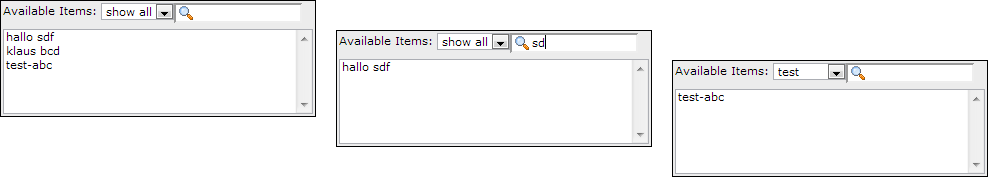
\includegraphics[width=1\linewidth]{Images/InDepthChanges/MultipleValueSelector.png}
	\end{figure}

\end{frame}

% ------------------------------------------------------------------------------
% Improved caching framework by introducing cache groups
% (slide added in March 2014)
% ------------------------------------------------------------------------------
% http://forge.typo3.org/issues/54991

\begin{frame}[fragile]
	\frametitle{Внутренние изменения}
	\framesubtitle{Группы кеширования (1)}

	\begin{itemize}
		\item Ядро TYPO3 использует два типа кешей:

			\begin{itemize}
				\item \textbf{системные}:
				кеш загрузки классов, кещ настроек, l10n\_cache, extbase\_object, extbase\_reflection и т. п.
				\item \textbf{кеши внешнего интерфейса}:
				cHash кеш, кеш страницы, кеш раздела страницы
			\end{itemize}

		\item В TYPO3 < 6.2, \textit{очистить все кеши} очищает \underline{все} кеши, что не идеально

		\item В TYPO3 >= 6.2, ядро использует две группы кешей:\newline
			"\textbf{страниц}" со всеми кешами к ним относящимися и "\textbf{системные}",
			используемые для кеширования компиляции и настроек

	\end{itemize}

	\begin{figure}
		
\includegraphics[width=0.5\linewidth]{Images/InDepthChanges/CacheGroups.png}
	\end{figure}

\end{frame}

% ------------------------------------------------------------------------------
% Improved caching framework by introducing cache groups
% (slide added in March 2014)
% ------------------------------------------------------------------------------
% http://forge.typo3.org/issues/54991

\begin{frame}[fragile]
	\frametitle{Внутренние изменения}
	\framesubtitle{Группы кеширования (2)}

	\lstset{
		basicstyle=\tiny\ttfamily
	}

	\begin{itemize}

		\item Связанные параметры настроек:\newline
			\smaller(в файлах: \texttt{LocalConfiguration.php}/\texttt{DefaultConfiguration.php})\normalsize

			\begin{lstlisting}
			'cache_hash' => array(
			  'frontend' => 'TYPO3\CMS\Core\Cache\Frontend\VariableFrontend',
			  'backend' => 'TYPO3\CMS\Core\Cache\Backend\Typo3DatabaseBackend',
			  'options' => array(),
			  'groups' => array('pages', 'all')
			),
			\end{lstlisting}

		\item Команда "\textit{Flush all caches}" более не очищает системные кеши
			(только "Clear Configuration Cache" или Install Tool очищают эти кеши)
		\item Новый параметр userTSconfig позволяет не администраторам очищать системыне кеши:\newline
			\smaller\texttt{options.clearCache.system = 1}\normalsize

		\breakingchange

	\end{itemize}

\end{frame}

% ------------------------------------------------------------------------------
% TCA: limit number of ticked checkboxes
% (slide added in March 2014)
% ------------------------------------------------------------------------------
% http://forge.typo3.org/issues/55187
% http://forge.typo3.org/issues/55188 (documentation: TCA reference)

\begin{frame}[fragile]
	\frametitle{Внутренние изменения}
	\framesubtitle{TCA: количество отмеченных флажков}

	\lstset{
		basicstyle=\tiny\ttfamily
	}

	\begin{itemize}
		\item TCA позволяет проверять количество отмеченных флажков

			\begin{itemize}
				\item \texttt{maximumRecordsChecked}:\newline
					предельное число записей в рамках всей системы
				\item \texttt{maximumRecordsCheckedInPid}:\newline
					предельное число записей в рамках PID (ID родителя)
			\end{itemize}

		\item Если внутренний пользователь достигает предельного значения, следующая галочка снимается,
		пока не будет снята какая-то другая

		\item Пример:

			\begin{lstlisting}
				$tcaConfiguration = array(
				  'type' => 'check',
				  'eval' => 'maximumRecordsChecked',
				  'validation' => array(
				    'maximumRecordsChecked' => 5
				  )
				);
			\end{lstlisting}

	\end{itemize}

\end{frame}

% ------------------------------------------------------------------------------
% TCA: Introduce MM_oppositeUsage property
% (slide added in March 2014)
% ------------------------------------------------------------------------------
% http://forge.typo3.org/issues/56061
% http://forge.typo3.org/issues/56123 (documentation: TCA reference)

\begin{frame}[fragile]
	\frametitle{Внутренние изменения}
	\framesubtitle{TCA: свойство \texttt{MM\_oppositeUsage}}

	\lstset{
		basicstyle=\tiny\ttfamily
	}

	\begin{itemize}
		\item При копировании записи \texttt{sys\_category}, создаётся новая связь MM, но без назначения "fieldname"
		\item Это значение обычно определяется из связанной сущности по \texttt{MM\_match\_fields}, но не может быть доступно
		\item Для разрешения этой проблемы, для TCA было представлено новое свойство \texttt{MM\_oppositeUsage}:

			\begin{lstlisting}
				'config' => array(
				  'allowed' => '*',
				  'MM' => 'tx_myextension_first_second_mm',
				  'MM_oppositeUsage' => array(
				    'tt_content' => array('somefield'),
				    'tx_myextension_domain_model' => array('some_property'),
				  ),
				),
			\end{lstlisting}

	\end{itemize}

\end{frame}

% ------------------------------------------------------------------------------
% Miscellaneous
% ------------------------------------------------------------------------------
% http://forge.typo3.org/issues/49037 (Custom record list in element browser)
% http://forge.typo3.org/issues/36505 (Increase size of be_groups.subgroup field)
% http://forge.typo3.org/issues/49270 (Merge extensions TS/Template)

\begin{frame}[fragile]
	\frametitle{Внутренние изменения}
	\framesubtitle{Дополнительно}

	\begin{itemize}

		\item \textbf{Список определенных записей:}\newline
			\small
				Список определенных записей можно использовать в проводнике по элементам,
				переназначив список записей элементов проводника по умолчанию.
			\normalsize

		\item \textbf{Дополнительные подгруппы:}\newline
			\small
				Атрибут \texttt{subgroup} в таблице БД \texttt{be\_groups} изменился из \texttt{varchar(250)} в \texttt{text}, что позволяет использовать более глубокую группировку (внутренних пользователей/групп)
			\normalsize

		\item \textbf{Объединение TS/Template в расширениях:}\newline
			\small
				Технически, "Веб > Шаблон" был разбросан по нескольким расширениям (tstemplate\_ceditor, tstemplate\_info,
tstemplate\_objbrowser and tstemplate\_analyzer). Теперь они объединены в одно единственное: "tstemplate"
			\normalsize

	\end{itemize}
	
\end{frame}

% ------------------------------------------------------------------------------
% Miscellaneous
% ------------------------------------------------------------------------------
% http://forge.typo3.org/issues/49721 (Add label_userFunc_options support to BackendUtility)
% http://forge.typo3.org/issues/50441 (Add a timestamp when downloading an extension)
% http://forge.typo3.org/issues/51352 (Force saltedpasswords for Backend)

\begin{frame}[fragile]
	\frametitle{Внутренние изменения}
	\framesubtitle{Дополнительно}

	\begin{itemize}

		\item \textbf{label\_userFunc\_option:}\newline
			\small
				Поддержка \texttt{label\_userFunc\_options} добавлена в \texttt{BackendUtility}
			\normalsize

		\item \textbf{Названия файлов расширений:}\newline
			\small
				При загрузке расширения через модуль управления расширениями, названия файлов содержат время (год, месяц, день и время):\newline
				\texttt{<extensionKey>\_<version>\_<timestamp>.zip}\newline
				\texttt{myextension\_1.0.0\_201312102359.zip}
			\normalsize

		\item \textbf{EXT:saltedpasswords:}\newline
			\small
				Расширение EXT:saltedpasswords стало обязательным, и теперь включено по умолчанию.
				Оно принудительно использует salted hashes для внутренней авторизации. Install Tool проверяет и,
				при необходимости подстраивает настройки.
			\normalsize

	\end{itemize}
	
\end{frame}

% ------------------------------------------------------------------------------
% Miscellaneous
% ------------------------------------------------------------------------------
% http://forge.typo3.org/issues/51138 (Allow SignalSlots to modify arguments)
% http://forge.typo3.org/issues/31996 (Transfer query parameters in preview)
% http://forge.typo3.org/issues/52630 (TCEforms PlaceHolder works recursively now)

\begin{frame}[fragile]
	\frametitle{Внутренние изменения}
	\framesubtitle{Дополнительно}

	\begin{itemize}

		\item \textbf{SignalSlots для изменения аргументов:}\newline
			\small
				Аргументы, переданные в диспетчер SignalSlots, теперь могут быть изменены, а диспетчер возвратит (измененные)
				аргументы в порядке получения, для сохранения последовательности в цепочке.
			\normalsize

		\item \textbf{Предпросмотр рабочей области:}\newline
			\small
				Теперь параметры запроса передаются при предпросмотре рабочей области. В TYPO3 < 6.2, была проблема, когда без передачи параметров, расширения работали неверно.
			\normalsize

		\item \textbf{TCEforms PlaceHolder возможность:}\newline
			\small
				Представленная в TYPO3 CMS 4.7, функция PlaceHolder для TCEforms теперь работает рекурсивно (например,
				\texttt{\_\_row|uid\_foreign|field}).
			\normalsize

	\end{itemize}
	
\end{frame}

% ------------------------------------------------------------------------------
% Miscellaneous
% ------------------------------------------------------------------------------
% http://forge.typo3.org/issues/14730 (Support for proxy NTLM authentication)
% http://forge.typo3.org/issues/49667 (Enable double-resolution icons in SpriteGenerator)

\begin{frame}[fragile]
	\frametitle{Внутренние изменения}
	\framesubtitle{Дополнительно}

	\begin{itemize}

		\item \textbf{Значки удвоенного разрешения:}\newline
			\small
				SpriteManager теперь поддерживают значки высокого разрешения: он формирует второй спрайт со значками удвоенного
				 разрешения (второй файл с суффиксом "@x2.png"). CSS3 удостоверяется, что файл высокого разрешения загружается на устройства с соответствующей поддержкой\newline
				(не затрагивая производительность других устройств).
			\normalsize

		\item \textbf{Аутентификация прокси NTLM:}\newline
			\small
				Поддержка аутентификации прокси NTLM (\textbf{NT} \textbf{L}AN \textbf{M}anager: набор протоколов безопасности Microsoft).  Функционал может быть включен Install Tool:\newline
				\normalsize
				\smaller
					\texttt{\$GLOBALS['TYPO3\_CONF\_VARS']['SYS']['curlProxyNTLM']}\newline
				\emph{(кстати: этот функционал запрашивался более 8 лет назад :-)}
			\normalsize

	\end{itemize}

\end{frame}

% ------------------------------------------------------------------------------
% Miscellaneous
% (slide added in March 2014)
% ------------------------------------------------------------------------------
% http://forge.typo3.org/issues/14730 (Support for proxy NTLM authentication)

\begin{frame}[fragile]
	\frametitle{Внутренние изменения}
	\framesubtitle{Дополнительно}

	\begin{itemize}

		\item \textbf{cookieHttpOnly по умолчанию:}\newline
			\small
				Для того, чтобы cookie сессии были доступны лишь через протокол HTTP,
				теперь по умолчанию \texttt{cookieHttpOnly} включено.\newline
				Это означает, что cookies "fe\_typo\_user" и "be\_typo\_user" недоступны для языков сценариев (например, JavaScript), что повышает защищённость против XSS атак (\textit{cross site scripting}). Но все же, некоторые старые браузеры не поддерживают подобной техники.
			\normalsize

		\item \textbf{Очистка таблицы БД:}\newline
			\small
				Из таблицы БД \texttt{tt\_content} удалены следующие атрибуты (не используемы со времён TYPO3 4.0):
				\texttt{text\_align}, \texttt{text\_face}, \texttt{text\_size}, \texttt{text\_color}, \texttt{text\_properties}.
			\normalsize

	\end{itemize}

\end{frame}

% ------------------------------------------------------------------------------
% Miscellaneous
% (slide added in March 2014)
% ------------------------------------------------------------------------------
% https://forge.typo3.org/issues/55190 (Move Tidy functionality to a TER extension)

\begin{frame}[fragile]
	\frametitle{Внутренние изменения}
	\framesubtitle{Дополнительно}

	\begin{itemize}

		\item \textbf{Удалён HTML Tidy:}\newline
			\small
				Функционал \textit{HTML Tidy} был удалён из ядра TYPO3. Он может быть с лёгкостью восстановлен установкой
				EXT:tidy из TER.
			\normalsize

		\item \textbf{Удалено dontSetCookie:}\newline
			\small
				Ввиду того, что cookie "fe\_typo\_user" устанавливаются лишь по необходимости (а не всегда), параметр Install Tool \texttt{dontSetCookie} потерял актуальность и был удалён.
			\normalsize

		\item \textbf{Удалены сценарии "мастеров":}\newline
			\small
				Удалены следующие сценарии "мастеров":
				\texttt{typo3/wizard\_add.php}, \texttt{typo3/wizard\_colorpicker.php}, \texttt{typo3/wizard\_edit.php}, \texttt{typo3/wizard\_forms.php}, \texttt{typo3/wizard\_list.php}, \texttt{typo3/wizard\_rte.php}, \texttt{typo3/wizard\_table.php}
			\normalsize

	\end{itemize}
	
\end{frame}

% ------------------------------------------------------------------------------

